\documentclass[border=4pt]{standalone}
\usepackage{amsmath,amssymb,tikz}\usetikzlibrary{arrows.meta}
\definecolor{figB}{RGB}{31,90,166}\definecolor{figR}{RGB}{176,48,48}\definecolor{figG}{RGB}{46,125,50}\definecolor{figO}{RGB}{214,120,20}
% v2 = (2,0), v1 = (0.5,1.2), c = 0.8: v1 + c v2 = (2.1,1.2). Both parallelograms have base v2 and height 1.2.
\begin{document}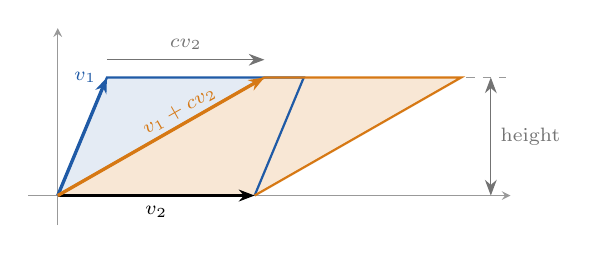
\begin{tikzpicture}[scale=1.25,>={Stealth[length=2mm]}]
\draw[black!40,thin,-stealth] (-0.3,0)--(4.6,0); \draw[black!40,thin,-stealth] (0,-0.3)--(0,1.7);
\draw[black!40,thin,dashed] (4.15,1.2)--(4.55,1.2);
\fill[figB!12] (0,0)--(2,0)--(2.5,1.2)--(0.5,1.2)--cycle;
\fill[figO!18] (0,0)--(2,0)--(4.1,1.2)--(2.1,1.2)--cycle;
\draw[thick,figB] (0,0)--(0.5,1.2)--(2.5,1.2)--(2,0);
\draw[thick,figO] (0,0)--(2.1,1.2)--(4.1,1.2)--(2,0);
\draw[->,very thick,black] (0,0)--(2,0) node[midway,below,font=\scriptsize]{$v_2$};
\draw[->,very thick,figB] (0,0)--(0.5,1.2) node[left,font=\scriptsize]{$v_1$};
\draw[->,very thick,figO] (0,0)--(2.1,1.2) node[pos=0.62,sloped,above,font=\scriptsize,inner sep=1.5pt]{$v_1+cv_2$};
\draw[->,thin,black!55] (0.5,1.38)--(2.1,1.38) node[midway,above,font=\scriptsize]{$cv_2$};
\draw[<->,thin,black!55] (4.4,0)--(4.4,1.2) node[midway,right,font=\scriptsize]{height};
\end{tikzpicture}\end{document}
